\chapter{Design and Implementation}\label{C:work}

A significant hurdle for the project was gaining enough understanding of the existing work on RBMs to be able to implement the ORBMs algorithm and architecture. This was crucial as an incorrect implementation invalidates Contributions \ref{item-c2} and \ref{item-c3} of this project.


\section{Implementation Design}

\subsection{Language Choice}

The implementation of the ORBM and inference algorithm is in \emph{Python}, with \emph{Matlab} and \emph{Java} being the other languages originally considered.

I have spent my university career working in Java, and nowdays it is efficient to perform machine learning tasks. Python's module and class system promotes composition, and multiple inherietance in particular allows for composition of different classes. Matlab is a popular numerical computing environment and has a lot of online resources as well as machine learing papers~\cite{hinton2006reducing} that include snippets or full Matlab programs that were used in the paper. Also Matlab is built around strong, efficient support for matrix operations which are very prolific in the RBM and ORBM implementations and evaluations.

Python has a very succinct syntax and shallow learning curve, as well as being the language of choice of my supervisor. This is favourable as I can have langauge level support for translating the algorithm into python correctly. Through libraries that supply wrappers for C-bindings, efficient code can be written in Python. Overall, being an interpreted language Python is slower than Matlab and Java. Three main factors outweighed this and resulted in the choice of Python:

\begin{description}
\item[Up front learning] Given the amount of up front learning of concepts required to implement the solution, Python was favoured over Java or Matlab because is has a very shallow learning curve. Despite having experience in Java as well as Python, I had never used machine learning or linear algebra libraries in either languages. Given the amount of up front learning required to understand the concepts in this project let alone implement it, I opted for the shallower learning curve of Python. Also my supervisor has experience using Python and the libraries involved with this project. A shallower learning curve meant that more time could be allocated to the evaluation which is the foremost contribution of this project.
\item[Library Support] Matlab and Python were two contenders in this factor, as a lot of matlab machine learning code is avaliable with supporting papers. Python has libraries such as NumPy, SciPy and Matplotlib~\cite{2015HistSciPy} which mirror Matlab functionality. However, NumPy and SciPy are all open source, while there is argument for treating an API as a black box --- i.e. not writing code that is dependant on the underlying implementation, having the option to view source helped me better grasp the concepts. In particular being able to compare my implementation of the RBM to  the Sklearn implementation~\cite{scikit-learn} allowed for some performance improvements to my implementation.
\item[Ease of Evaluation] Python provides a strong plotting library that is inspired by Matlab and R --- MatplotLib. Matplotlib is interoperable with the NumPy library, meaning that visualising results was really easy.

Also the evaluation requires repeatedly running a test to gain more confidence in the stochastic result. This is made possible by the ECS-Grid. Python only required a simple script that manages input and output. However the Java support on the ECS grid requires significantly more setup. This seemed like an unnecessary risk to introduce to the project at the later stage when the evaluation would being carried out.
\end{description}
%
% All of the languages considered have the efficiency for machine learning tasks, despite Python being on the slower end of the spectrum of languages, versus that of the compiled JVM languages like Matlab or Java, it is still fast enough. The complexity of the traditional RBM is relative to what is trying to be modelled, less of the language implementing it.
% Java and Python have robust testing suites given they are used for non-academic goals. Matlab and R do have suites however the author has not had experience with them. Choosing from one of these two languages would increase the amount of upfront learning required and therefore increase this risk.
% The author had the most experience with Python and Java, however Python was favoured due to it's Matlab-like library NumPy. Expressive matrix syntax combined with the familiarity and brevity of Python made it a compelling option.


\subsection{Program Architecture}

The implementation of the RBM, ORBM and algorithm is implemented with unit testing and composability in mind. It is important that the design supports comparing the Full and Approximated Correction (Equations~\cite{eq:Full-Corretion} and ~\cite{eq:Approx-Correction}. By using Python, multiple inheritance could be leveraged to achieve this composability. For instance adding support for continuous pixel values to the \texttt{Full Correction Sampler}, one simply needed to extend \texttt{Continuous Approximate Correction Sampler} and the \texttt{Full Correction Sampler}, with no code actually in the new class. The architecture is pictured in the class diagram \ref{F:Prog-Arch}. There were three main roles these classes filled:
\begin{enumerate}
  \item The \texttt{Trainer} was used to train the weights of a supplied \texttt{RBM}. It would do so using a supplied \texttt{sampler}, decoupling how samples were generated from the training process.
  \item The \texttt{RBM} was the model of an RBM, storing the weight matrix, as well as parameter information. Also this supported conversion of the SciPy Sklearn libraries' RBM implementation into the implementation used in this project. Decoupling the concept of an \texttt{RBM} from the \texttt{Sampler} and the \texttt{Trainer} meant that RBMs could be `plugged' into the ORBM architecture with ease.
  \item The \texttt{Sampler} defined how to perform Gibbs sampling, the subclasses defining whether it is standard RBM sampling or ORBM sampling. This made it trivial to compose \texttt{samplers}, which was required for the ORBM samplers.
\end{enumerate}

\begin{figure}[h]
\begin{center}
  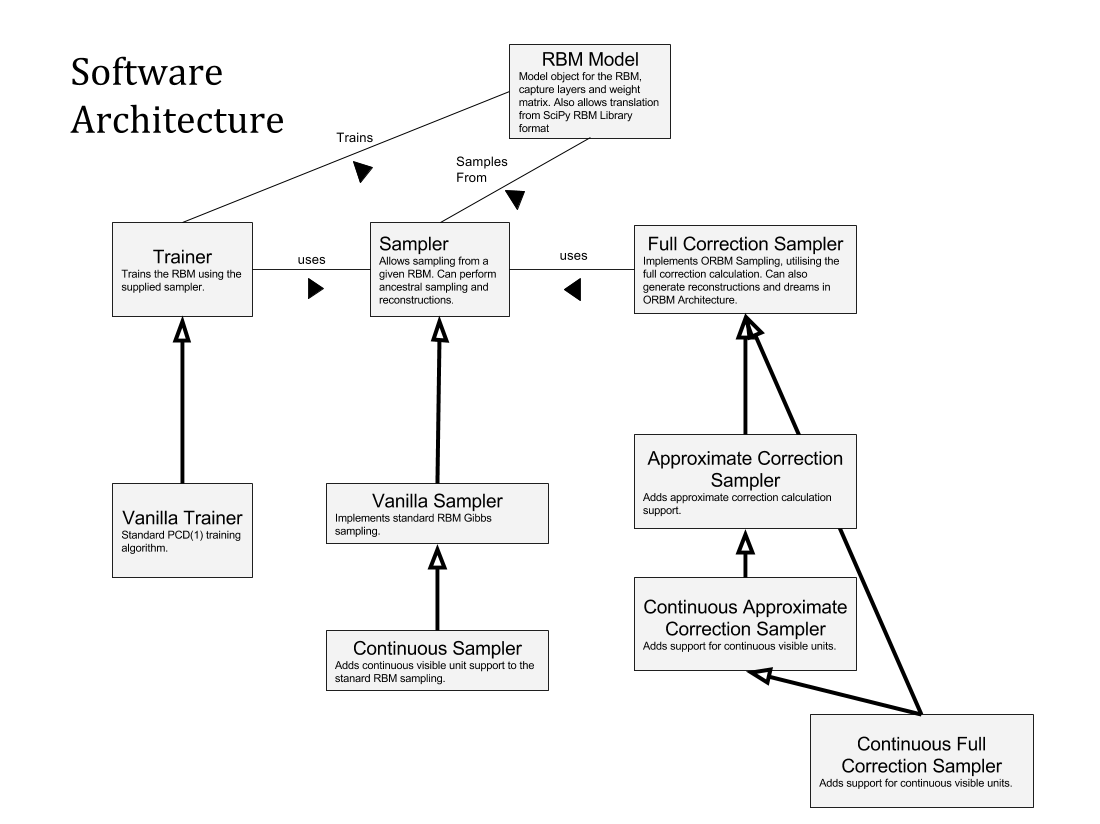
\includegraphics[width = 1\textwidth]{Assets/ENGR489-Architecture.png}
\caption{A figure showing the architecture for the implemented test suite in UML notation.}
\label{F:Prog-Arch}
\end{center}
\end{figure}

\subsection{Testing Approach}

The inference algorithm is the most crutial part of the implementation to test. In larger dimensional tasks, unit testing to ensure the algorithm produces the correct values becomes difficult. In smaller cases I was able to ensure the probabilities of $P(h|v)$ and $P(v|h)$ calculated by the implementation matched calculations I made by hand. Being an unsupervised black boxes, determining if an RBM (and by extension the ORBM) hidden representation is `correct` for larger tasks such as the MNIST handwritten digit dataset is non-trivial. Concerned by this risk, I designed my evaluations to build confidence in the algorithm and the implementation.

\section{Evaluation Design}
\subsection{Examining the mixing time of inference in the ORBM}

As described in Section \ref{S:ORBM-Inference}, sampling from $h^A$ and $h^B$ suffers from the effect of explaining away (Section \ref{S:Explaining-Away}) which requires a Gibbs chain to be run. While intractable for a large SBN, as only two causes are being modeled, ideally the Gibbs chain for this process won't take many iterations to mix. As the correction needs to be computed for each Gibbs iteration, a long Gibbs chain could be detrimental to performance.
Finding this \emph{optimal mixing time} for the ORBM is only an issue as the number of dimensions and training examples increase. In smaller dimensions mixing can be overcome by using a large ($>1000$) number of Gibbs iterations, as it computational feasible to do so. However in the larger problems this becomes intractable, so an optimal mixing time is desired.

This project examines the mixing time by way of examining reconstructions at various points of the Gibbs chain. This is also interesting in that we can observe the dynamics of the network and the effect of applying the \emph{correction} has on reconstructions. Hinton~\cite{Hinton-Animations} has had success observing reconstructions in an animated setting.

\subsection{Evaluating RBMs and ORBMs}

  A challenge faced by this project and work with RBMs is that they are non-trivial to evaluate. Being an unsupervised black box, one cannot merely inspect the hidden units sampled after a given input and be sure that a good model has been learnt. As I plug RBMs into the ORBM architecture it is important for the overall results that the RBMs are well trained.

\subsection{Hinton diagrams}
  We can examine the weights into a given hidden unit in the shape of the visible vector. For instance in the context of images, \texttt{Hinton Diagrams} allow visualisation of what a given hidden unit is `doing' by visualising the matrix of weights into that unit. This was first used by Hinton in the context of Boltzmann Machines in~\cite{Hinton:1986:LRB:104279.104291}. They also give insight into hidden unit utilisation. Weights are often initialised to small random values resulting in a Hinton diagram with little structure to it. This is illustrated in figures \ref{F:Hinton-Good} and \ref{F:Hinton-Bad}. The former showing a hidden units weights where some structure has been learnt, and the latter showing the opposite.

  \begin{figure}[htb]
  \centering
  \begin{subfigure}[t]{0.3\textwidth}
      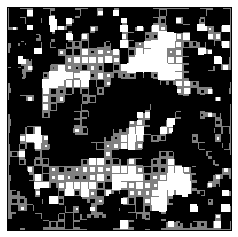
\includegraphics[width=\textwidth]{Assets/HINTON1.png}
      \caption{Utilised hidden unit Hinton Diagram}
      \label{F:Hinton-Good}
  \end{subfigure}
  ~ %add desired spacing between images, e. g. ~, \quad, \qquad, \hfill etc.
    %(or a blank line to force the subfigure onto a new line)
  \begin{subfigure}[t]{0.3\textwidth}
      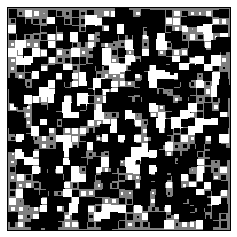
\includegraphics[width=\textwidth]{Assets/HINTON2.png}
      \caption{Unutilised hidden unit Hinton Diagram}
      \label{F:Hinton-Bad}
  \end{subfigure}
  \caption{Hinton Diagrams illustrating a trained hidden unit, versus that of an untrained/unutilised hidden unit. This is with no measures to enforce sparsity.}\label{fig:mnist-worse-best-results}
\end{figure}

\subsection{Reconstructions: a measure of performance}

Reconstructions, as described in Section \ref{SS:RBM-Reconstructions}, are a good measure of performance. Reconstructions will be the main way I evaluate the RBM in comparison to the ORBM. To be able to use this reconstruction based evaluation, knowledge of the ground truth is required. This is so:
\begin{itemize}
  \item RBMs could be trained and then plugged into the ORBM network.
  \item Reconstructions could be compared directly (by score) to the ground truth.
\end{itemize}

\subsection{Evaluating RBMs: Problem dependent}

  Evaluating RBMs is problem dependent, we can examine the different approaches available by splitting problems into two classes:
  \begin{description}
  \item[Problems with small dimensionality] When the dimensionality of the input is very small ($<10$) and all possible inputs are known, we can perform analytical evaluations of the RBM. By clamping the visible units of the RBM to each input in the training set, reconstructions can be created. This process can be repeated for each input, recording the frequency that each reconstruction occurs on a bar graph. We can then ensure that the RBM is reconstructing the input perfectly.

  In a similar way to the reconstructions, samples can be drawn from RBM in a `free phase` without the input clamped to a given visible. The bar graph should exhibit dream visible patterns from the whole training set approximately an equal proportion to that of the training set.

  \item[Problems with large dimensionality] In non-trivial cases, with larger datasets, reconstructions can be inspected and compared to the training dataset. However, empirically detecting if a model is trained is difficult, especially given the unsupervised, black box nature of RBMs.
  Alternatively, a `score` can be assigned to each item in the training set based on how well the RBM can reconstruct it.
  This project will use two scores the \emph{Cross Entropy}~\cite{golik2013cross} and the \emph{Negative Cosine Angle} to compare the reconstructions to the ground truth images.
  Dreams can also be examined in larger cases, but empirically detecting if they are `correct' is infeasible. Nevertheless, Dreams are useful to examine, as if they look like items in the training set, this gives confidence the RBM is capturing the model.

\end{description}

All evaluations followed the same high level process, working from trivial cases to more challenging tasks. By changing only a few aspects from problem to problem it allows me to identify what qualities of the problem make the algorithm less or more effective. These asepcts were typically the dimensionality and then ultimately the difficultly of the problem. The justification for this being that trivial cases make unit testing feasible, therefore ensuring conclusions can be drawn with regard to the algorithm and model, not an incorrect implementation.

The evaluations in this project aimed to evaluate the ORBM and it's inference algorithm by examining reconstructions given a multi-cause image. Because the multi-cause inputs were images composed of known images, I could then compare the reconstructions to the ground truth. An example of a multi-cause input with two quadrilaterals is shown in Figure \ref{F:Composite-Example}. The optimal reconstructions are equivalent to the two images that combined form the input.

\begin{wrapfigure}{r}{0.6\textwidth}
  \begin{center}
    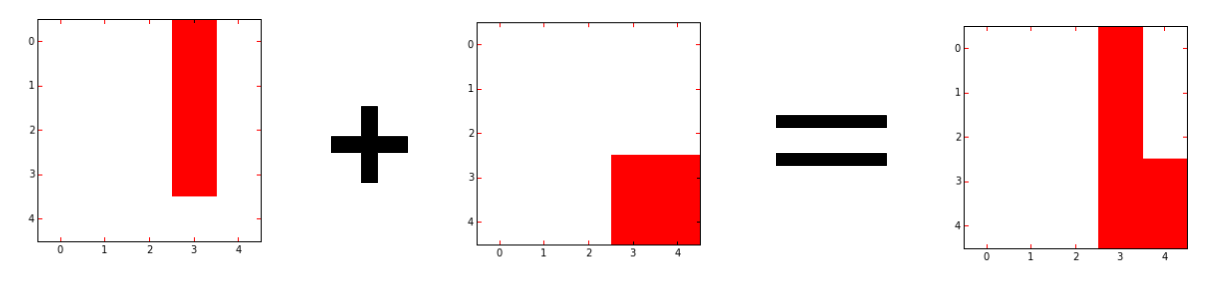
\includegraphics[width=0.48\textwidth]{Assets/Composite-Example.png}
  \end{center}
  \caption{A figure illustrating two five by five pixel images combining to form a composite/multicause input. The images are binary.}
  \label{F:Composite-Example}
\end{wrapfigure}

In the smaller dimensional cases the reconstructions are inspected by plotting the reconstructions and the frequency with which they occurred after a large amount of repetitions. In the larger dimensional tasks, the two `scores' are used to evaluate reconstructions against the corresponding item of the training set.


\subsection{Choice of Evaluation Datasets}

As my evaluations follow the same outline of training RBMs, plugging them into the ORBM, and evaluating the reconstructions, the key aspect of the evaluation that needs to be designed is the datasets for these tasks. It is important the images of the datasets are \emph{multi-subject} and that the individual images used to compose the training images are known. This is to allow the reconstructions of the ORBM (and RBM) to be compared to these underlying images, exploring how well the ORBM and RBM can perform source separation.

\begin{description}
  \item[2 Bit XOR] The minimal case of image source separation. The RBMs are trained on a single bit being on in a two bit pattern. The training set then resembles a 2 bit XOR truth table. Because the dimensions of this task are so small, reconstructions and dreams can be evaluated empirically. Also the algorithm can be unit tested ensuring the outputs of the different steps are correct, comparing them to values calculated by hand. Also as the dimensionality is so small, the Approximated Correction and the Full Correction can be compared to ensure that the approximated correction works well in practice.
  \item[$X$ neighboring bits on in $Y$ bit pattern] This is a natural next step from 2 bit XOR, and is effectively the same task but in larger dimensions. It is trivial to train an RBM to represent this problem, and the algorithm is quick to run on such a small dimensionality creating a quick feedback loop for development.
  \item[2 by 2 squares in a 5 by 5 pixel image] This dataset extends the previous increasing to 25 dimensions. The dataset is trivial to construct and corresponds to a square of 2 by 2 pixels being on in a 5 by 5 pixel image. Interesting cases can be explored and then inspected visually as images, which are easier to interpret than bit strings (especially as the bit strings get larger than 10).
  \item[Rectangles in a 5 by 5 pixel image] This dataset builds on the previous by introducing different shaped \emph{subjects} to the images. This means that two RBMs need to be trained, one for each subject. This dataset, much like the previous allows for compelling cases to be separated. It sets the scene for the larger dimension cases.
  \item[MNIST Handwritten Digit Dataset] This is a prolific machine learning dataset~\cite{mnistlecun}. By using the dataset in this project it aids in reproducibility and as there has been previous work it is known that RBMs can be trained successfully on the data. The dataset is comprised of 28 by 28 pixel handwritten digit images, where a pixel value is between 0 and 1. There are digits 0 through 9. To make a multi-cause input, each digits it is composed with every other digit, making the novel, yet non-trival task of separating two digits from a single image.
\end{description}
